\chapter{Lecture 29 - Loss of Coolant Accident}
\label{ch:ch29}
\section{Objectives}
The objectives of this lecture are:
\begin{enumerate}
\item Review containment design requirements
\item Discuss factors to consider for coolant system ruptures as it applies to containment design
\item Describe the control volume approach to LOCA containment analysis
\end{enumerate}

\section{Containment Design Requirements}

\begin{marginfigure}
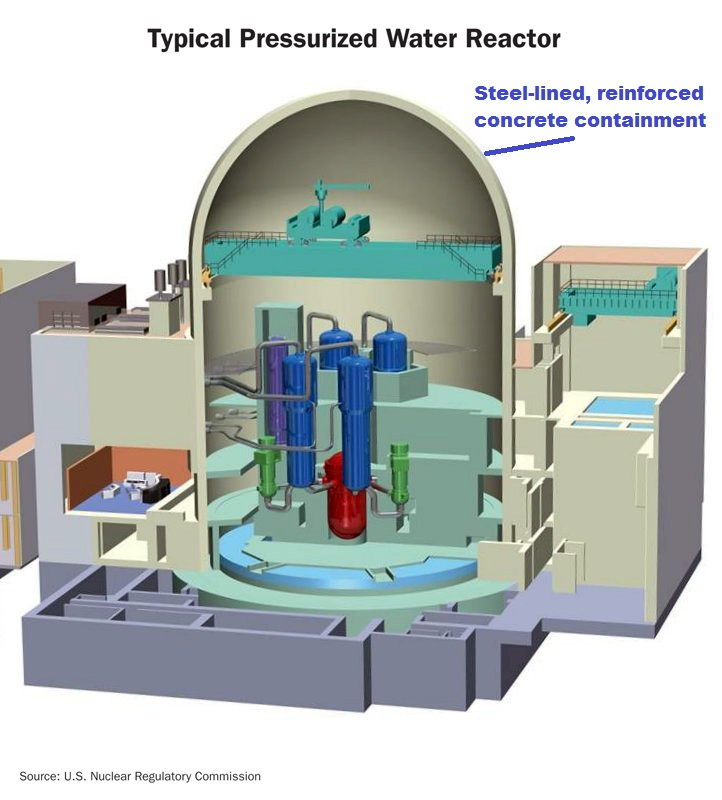
\includegraphics{pwr-containment.png}
\caption{Containment for typical PWR.}
\label{fig:pwr-containment}
\end{marginfigure}
The containment for a nuclear reactor has several functions.
\begin{itemize}
\item \emph{Public \& Environmental Protection.} As the name ``containment'' implies, one of it's chief functional requirements is to prevent release of radioactivity to the environment.  In the event that a radiological release becomes inevitable, a secondary requirement is to prevent the \emph{large early} release of radioactivity.  If the release is not large or if it comes with ample warning, emergency planning measures can be put into effect to minimize damage and danger to people.

\begin{marginfigure}
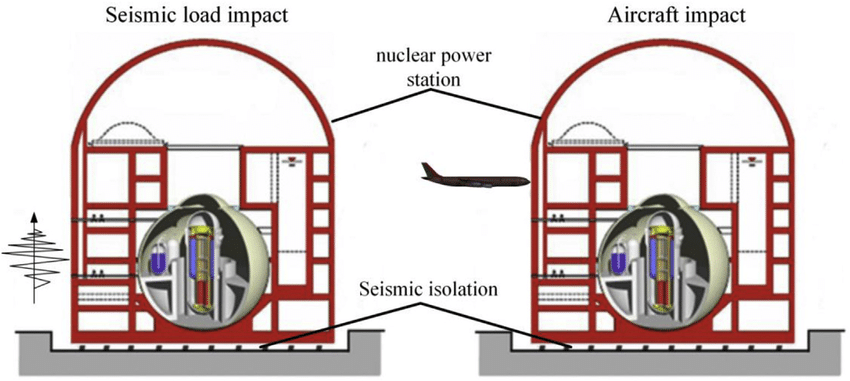
\includegraphics{seismic-and-impact.png}
\caption{Containments must withstand seismic and impact loads.}
\label{fig:seismic-and-impact}
\end{marginfigure}
\item \emph{Protection of Plant Systems.}  Nuclear power plant systems are not especially vulnerable and yet, like all industrial equipment, they must be protected from the elements under ordinary circumstances; protected from fires and floods in unusual circumstances.  After the 9/11 attacks, additional emphasis was added to protection against human actions: crashing airplanes, explosives, and acts of sabotage.  Whatever the threat, the stakes of damage to nuclear power plant systems is somewhat higher than a typical industrial building so additional design features---or at least additional design analysis---to ensure the nuclear systems have protection against foreseeable natural and man-made hazards are needed.

\item \emph{Structural Support of Systems.}  These loads include:
\begin{enumerate}
\item \textbf{routine service loads:}  Structural support of the reactor vessel and primary coolant systems.  Lifting and handling equipment must be installed to support refueling and expected maintenance activities.  
\item \textbf{seismic loads:} Depending on geographic location, seismic loads may or may not qualify as ``routine'', but earthquakes small as well as large must be accounted for in the design of the reactor containment as well as nuclear system support structures.

\begin{marginfigure}
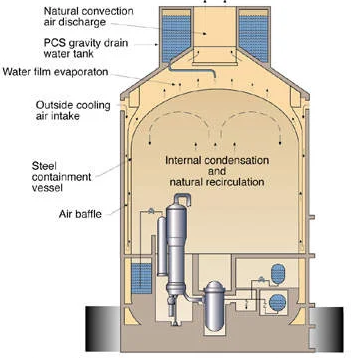
\includegraphics{AP1000-containment.png}
\caption{AP1000 containment schematic.}
\label{fig:AP1000-containment}
\end{marginfigure}

\item \textbf{Internal loads during design basis accidents.}  Perhaps this is a repeat of the ``containment'' function, but it is worth emphasizing that design basis accidents like loss of coolant accident (LOCA) and steam line rupture (SLR) accidents result in significant structural and thermal loads on the containment boundary that the containment must be designed to withstand.
\end{enumerate}
\end{itemize}  
Our current focus for this lecture is to quantify the consequences of a LOCA from a containment design perspective.

\section{LOCA Containment Analysis}
\newthought{In the event} that there is a large loss of coolant accident, the engineer must ensure that the containment structure will be able to withstand the temperature, pressure, and, in the case of water-cooled reactor LOCA, humidity of the post-accident environment in the containment.

Some factors to consider in this analysis include:
\begin{itemize}
\item \emph{Possible heat sources.} These heat sources include:
\begin{enumerate}
\item \textbf{Stored heat in the reactor system fluids.}  For a PWR the primary coolant system is at high temperature and pressure.  After the LOCA, one can expect the mass/energy of the primary coolant to expand into the entire containment system.  
\item \textbf{Decay heat.}  Even if control rods, or other reactivity control systems, are successfully employed to promptly shut down the reactor, decay heat will remain.  The magnitude of the decay heat will depend on the operating history of the reactor but this significant energy source must be included in any realistic analysis.
\item \textbf{Exothermic chemical reactions.}  These reactions include:
\begin{enumerate}
\item for LWRs, high-temperature oxidation of Zircaloy cladding in the presence of water.  In addition to releasing heat, hydrogen is a product of this reaction.
\item for sodium-cooled reactors: oxidation of the sodium coolant in the presence of air and/or water.
\item for carbon-dioxide-cooled reactors: oxidation of the graphite moderator by the carbon dioxide coolant.
\item for all reactors: oxidation of metals that may exist in molten core material (``corium'') by water and carbon dioxide released from thermal decomposition of the concrete containment basemat on contact with the corium.
\end{enumerate}
\end{enumerate}
\item \emph{Possible heat sinks.} These include:
\begin{enumerate}
\item Containment walls and other surfaces that are able to store energy.
\item active containment heat/pressure mitigation systems such as:
\begin{enumerate}
\item air coolers
\item sprays
\item endothermic chemical reactants
\item built-in emergency cooling systems
\end{enumerate}
\end{enumerate}
\item \emph{Fluids added from external sources}.  Perhaps this can be categorized under ``heat sinks,'' but the containment design analysis might consider the mitigating effects of providing additional cooling fluids into the containment environment after the accident has occurred.  These might include additional core cooling water or, in the case of a BWR, additional feedwater.
\end{itemize}

\section{Analysis Approach for LOCA}

\newthought{Let us consider} the containment and everything inside of it as a fixed control volume.  Upon initiation of the LOCA, the high pressure and temperature fluids inside the reactor coolant system interacts with and, eventually come into mechanical and thermal equilibrium with the air in the containment.  

If we consider this as any other thermodynamic process between an initial and final state point we might first write down a statement of conservation of energy.  

\begin{multline}
m_{\text{air}}u_{\text{air}_1} + m_{w}u_{w_1} + m_{w,\text{air}}u_{w,\text{air}_1} + Q_{1 \rightarrow 2} = \\ m_{\text{air}}u_{\text{air}_2} + m_{w,\text{air}}u_{w,\text{air}_2} + m_w u_{w_2}
\label{eq:loca-coe}
\end{multline}
where $m_{\text{air}}$ is the mass of air in the containment, $m_{w}$ is the mass of water in the primary coolant system, $m_{w,\text{air}}$ is the mass of water in the air in the containment,\sidenote{We assume that the air in the coolant initially has some humidity.  Admittedly, this is a small detail and does not greatly impact the results of the analysis, but it is included in the treatment by Todreas, so I will include it here.} and $Q_{1 \rightarrow 2}$ is the heat that passes the control volume boundaries during the process.  The temperature-entropy plot for the water in shown in Figure \ref{fig:ts-water-loca}.  The temperature-entropy plot for air is shown in Figure \ref{fig:ts-air-loca}.
\begin{marginfigure}
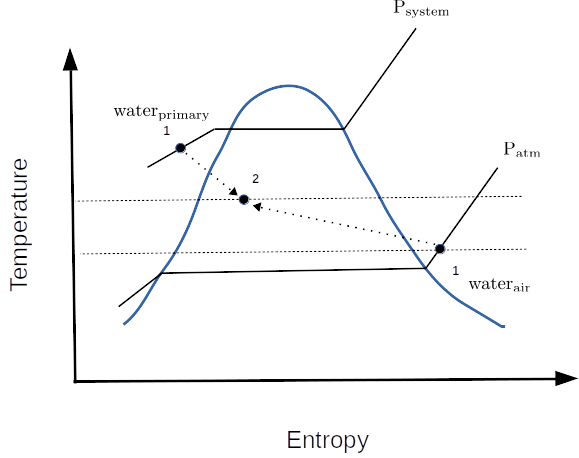
\includegraphics{ts-water-loca.png}
\caption{Temperature-Entropy plot for Water in a LOCA.}
\label{fig:ts-water-loca}
\end{marginfigure}

\begin{marginfigure}
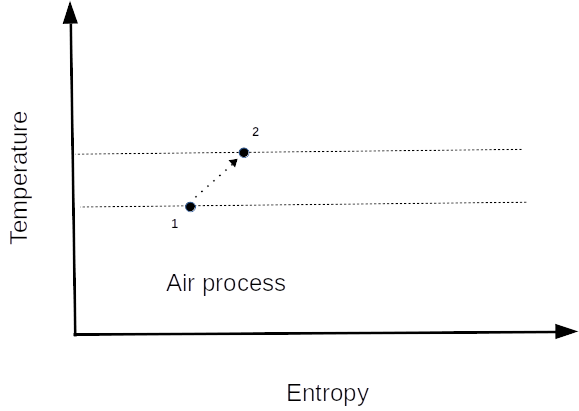
\includegraphics{ts-air-loca.png}
\caption{Temperature-Entropy plot for Air in a LOCA.}
\label{fig:ts-air-loca}
\end{marginfigure}
In addition to the energy equation provided in Equation \ref{eq:loca-coe}, we will assume that the overall containment volume will remain fixed:

\begin{equation}
V_{\text{final}} = V_{\text{reactor coolant}} + V_{\text{containment}}
\label{eq:cov-loca}
\end{equation}
and we will assume the final static pressure to be equal to the partial pressure due to water (or water vapor) plus the pressure of the air:
\begin{equation}
P_{\text{final}} = P_{\text{air,final}} + P_{\text{water,final}}
\label{eq:cov-loca}
\end{equation}
Lastly we will assume that the air and water within the containment volume come to thermal equilibrium:

\begin{equation}
T_{\text{air,final}} = T_{\text{water,final}}
\label{eq:loca-thermal-eq}
\end{equation}

\section{Basic Analysis Method}
In this section, we will consider the case where humidity in the containment air is not considered.  The following steps are taken:

\begin{enumerate}
\item Determine the initial mass of water in the primary and mass of air in the containment volume.  There are a number of ways the problem can be posed, but let us assume that these values are either given or can be easily computed with given data.

\item Calculate the \emph{final} specific volume of water in the containment volume.  We will assume that mass does not cross the system boundaries---i.e. no water or air is allowed in or out of the containment boundary.  We have the water mass from the previous step; we get the final volume from Equation \ref{eq:cov-loca}, so we can compute the specific volume.

\item Begin an iterative process to find the final temperature:
\begin{enumerate}
\item Guess final temperature.
\item With this trial temperature and the (constant) specific volume of the water, we can determine the pressure and internal energy of the water.
\item With the same trial temperature, compute the pressure and internal energy of the air.

\item Check the energy balance given by Equation \ref{eq:loca-coe}.  Note that this steps requires that we specify how much energy is transferred in or out of the system.  As a starting point, it is often useful/reasonable to assume no energy enters or leaves the system.\sidenote{A refinement would be to assume energy is added due to decay heat; one could then treat the problem as a quasi-steady-state system in which we find the ``steady state'' after, say 1 hour of decay heat addition; then another ``steady state'' after 2 hours (etc...).  Another refinement would be to consider adding water from emergency core cooling systems to the system; yet another might consider energy dissipation due to endothermic chemical reactions or heat transfer through the containment boundary.}
\item Adjust your temperature guess based on the energy balance and repeat until you converge to a temperature at which the energy balance is satisfied.
\end{enumerate}
\end{enumerate}
Complete MATLAB code to carry out this analysis is provided in the appendices.

\section{Final Comments}
\newthought{The point} of this lecture is to help you answer, or at least partially answer, the questions: \emph{``How big should my containment be?''} and \emph{``How thick should my containment walls be?''}  If we simply view the containment as a pressure vessel, sized so as to satisfy all of the non-accident functional requirements, we can use the final containment temperature and pressure to find necessary containment wall thickness.  If we make the containment bigger, we expect a lower final pressure on a LOCA; if smaller: higher pressure and temperature after the LOCA.  If we want to specify a maximum temperature or pressure post-LOCA, we can use the methods to determine how big the containment should be.  This is a question that often gets left out of textbook treatments of this topic, but the tools to do at least a simple analysis are available to you; you should use them. 

